Como valores iniciales de las variables no observadas escogimos distintas opciones para asegurarnos de que no haya diferencia en los valores a los cuales convergen. Para los gráficos expuestos se utilizaron los siguientes parámetros para el algoritmo de muestreo.

\begin{lstlisting}[frame=single]
% Sampling
% MCMC Parameters
nchains = 2; % How Many Chains?
nburnin = 10e2; % How Many Burn-in Samples?
nsamples = 10e4;  %How Many Recorded Samples?
nthin = 1; % How Often is a Sample Recorded?
doparallel = 0; % Parallel Option

% Assign Matlab Variables to the Observed Nodes
datastruct = struct('k1',k1,'k2',k2,'k3',k3,'n',n);

% Initialize Unobserved Variables
for i=1:nchains
    S.theta1 = 0.5; % Intial Value
    S.theta2 = 0.5; % Intial Value
    S.theta3 = 0.5; % Intial Value
    S.alpha = randi([1 3]); % Intial Value
    init0(i) = S;
end

\end{lstlisting}

\subsection{Histogramas}

\begin{figure}[H]
\begin{minipage}{1.0\textwidth}
 \centering
	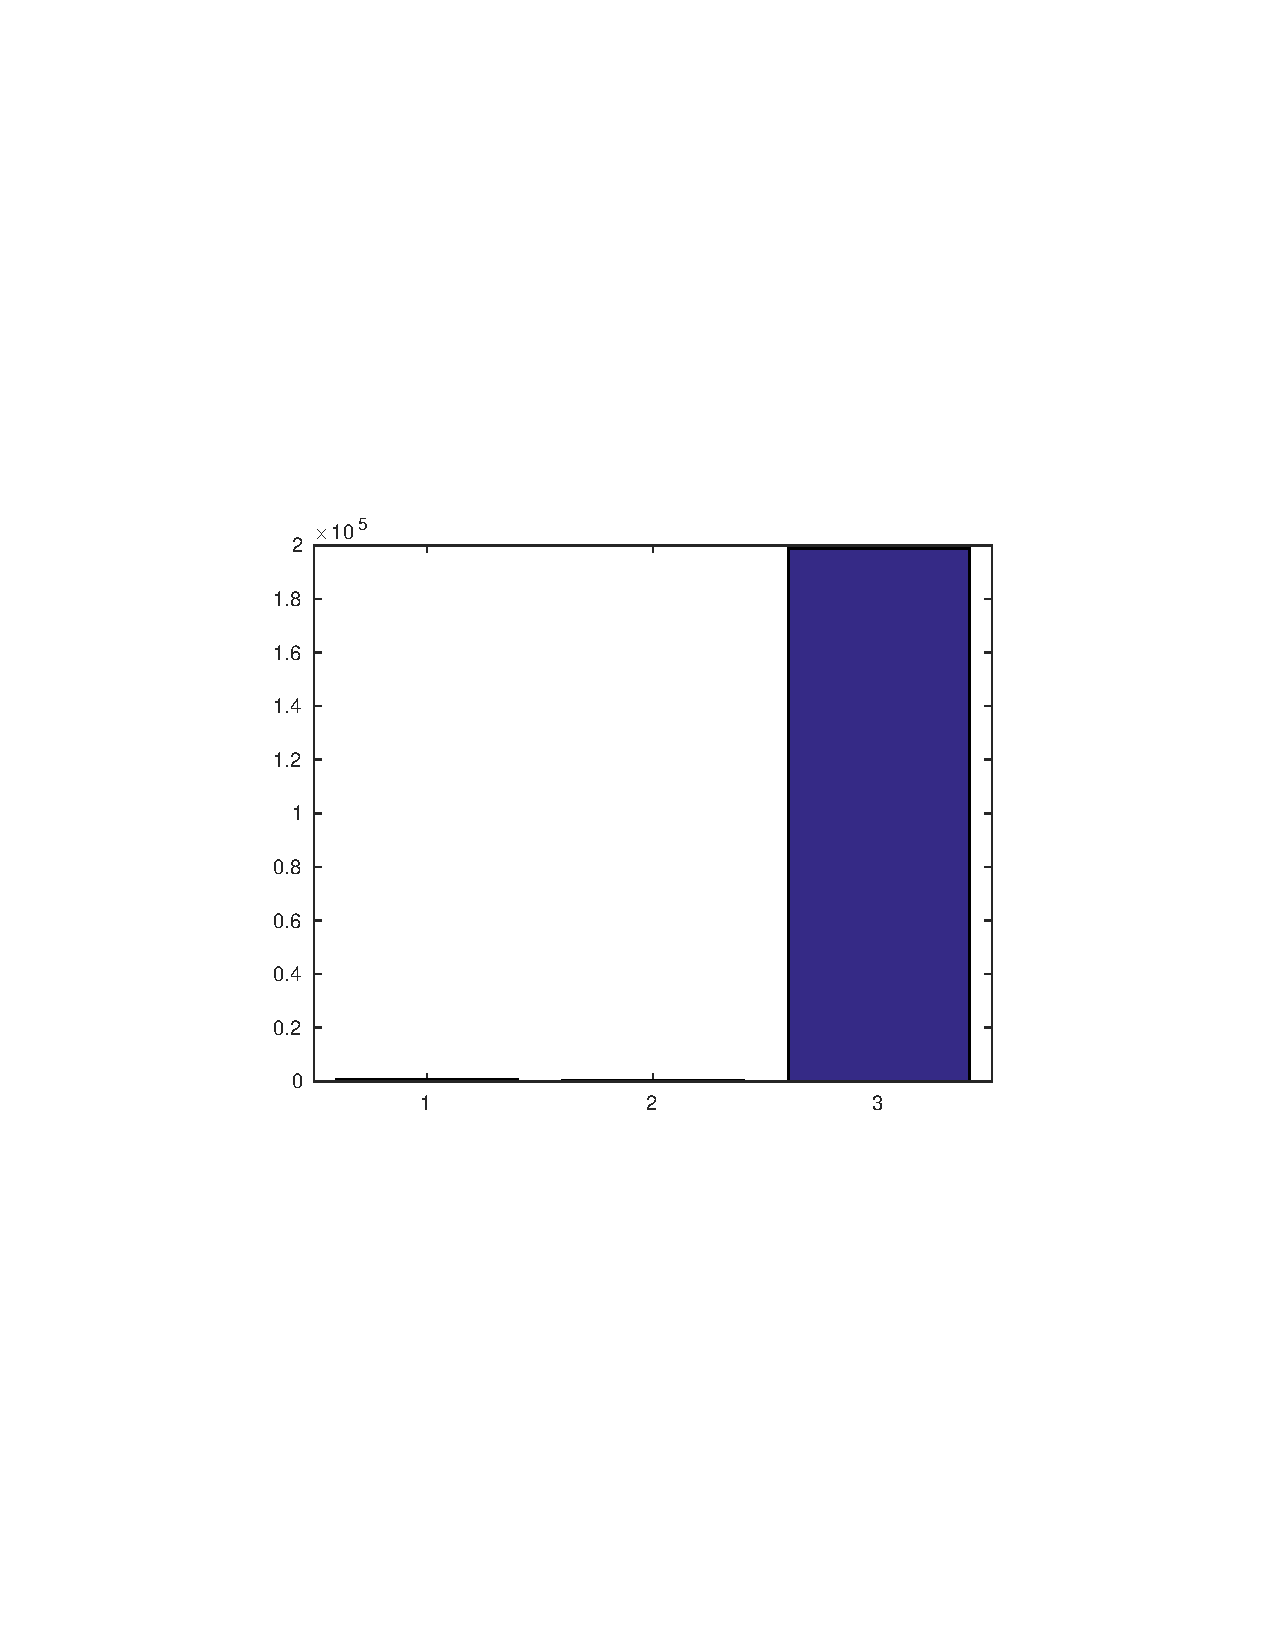
\includegraphics[width=0.8\textwidth]{imgs/alpha.pdf}
	\caption{\footnotesize Histograma de la variable $\alpha$.}
\end{minipage}
\end{figure}

\begin{figure}[H]
\begin{minipage}{1.0\textwidth}
 \centering
	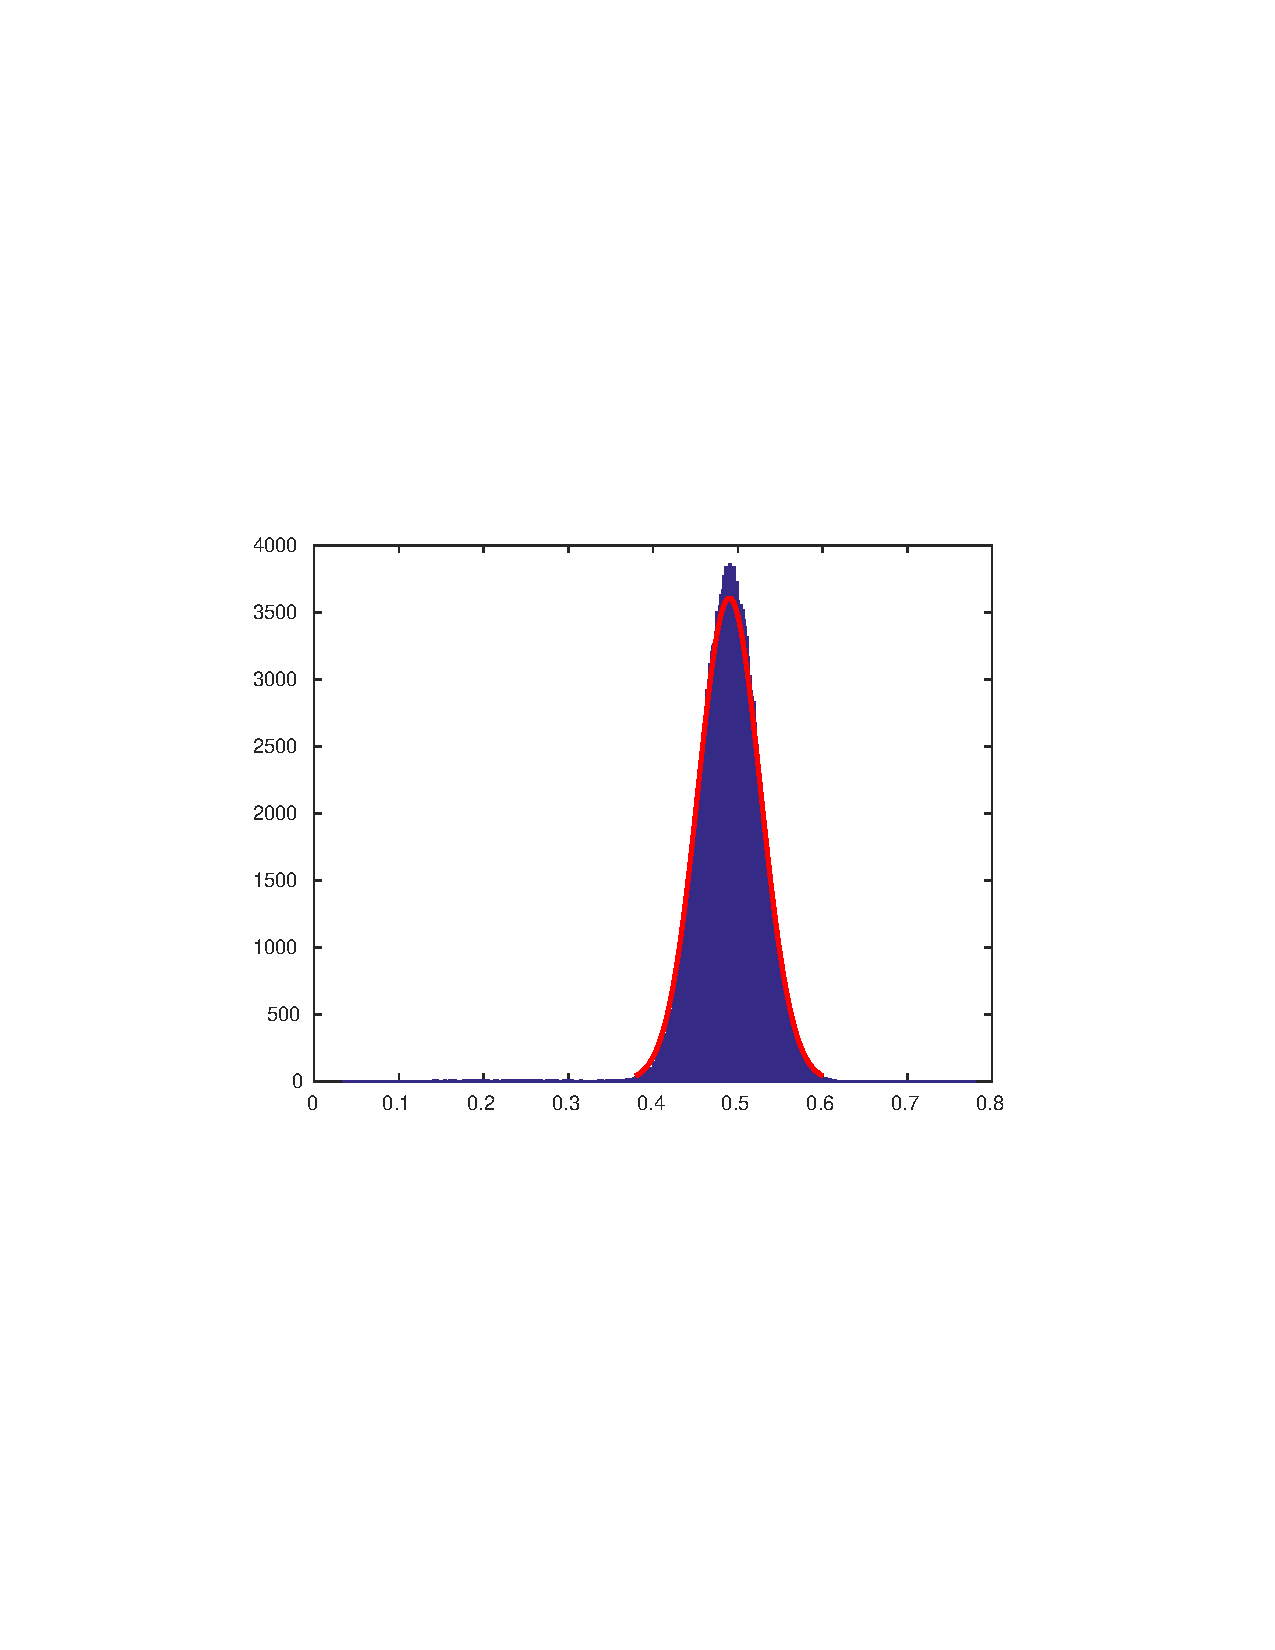
\includegraphics[width=0.8\textwidth]{imgs/theta1.pdf}
	\caption{\footnotesize Histograma de la variable $\theta_1$. La linea roja es una aproximacion con una distribución normal.}
\end{minipage}
\end{figure}

\begin{figure}[H]
\begin{minipage}{0.45\textwidth}
 \centering
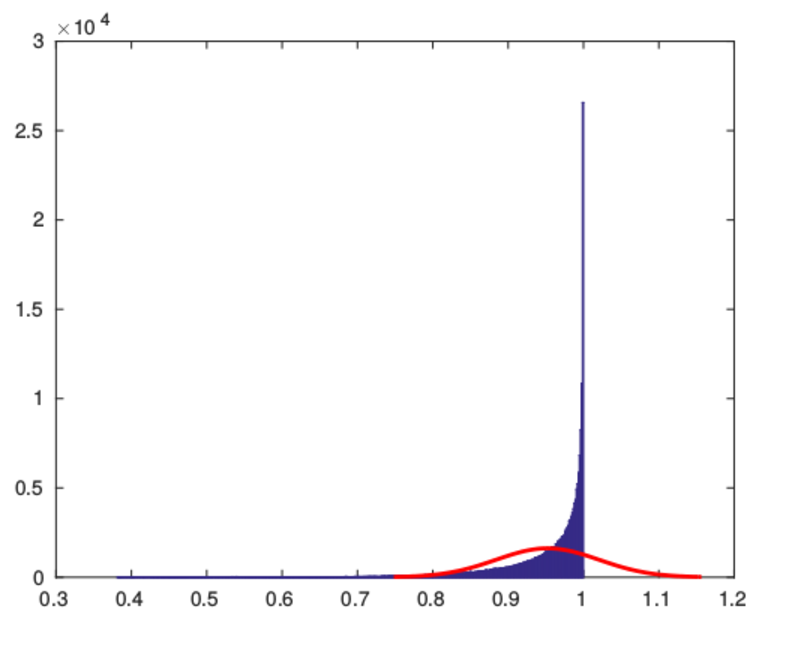
\includegraphics[width=1.0\textwidth]{imgs/theta3.pdf}
	\caption{\footnotesize Histograma de la variable $\theta_3$. La linea roja es una aproximacion (Poco precisa como se podrá observar)con una distribución normal.}
\end{minipage}
\hspace{0.1\textwidth}
\begin{minipage}{0.45\textwidth}
 \centering
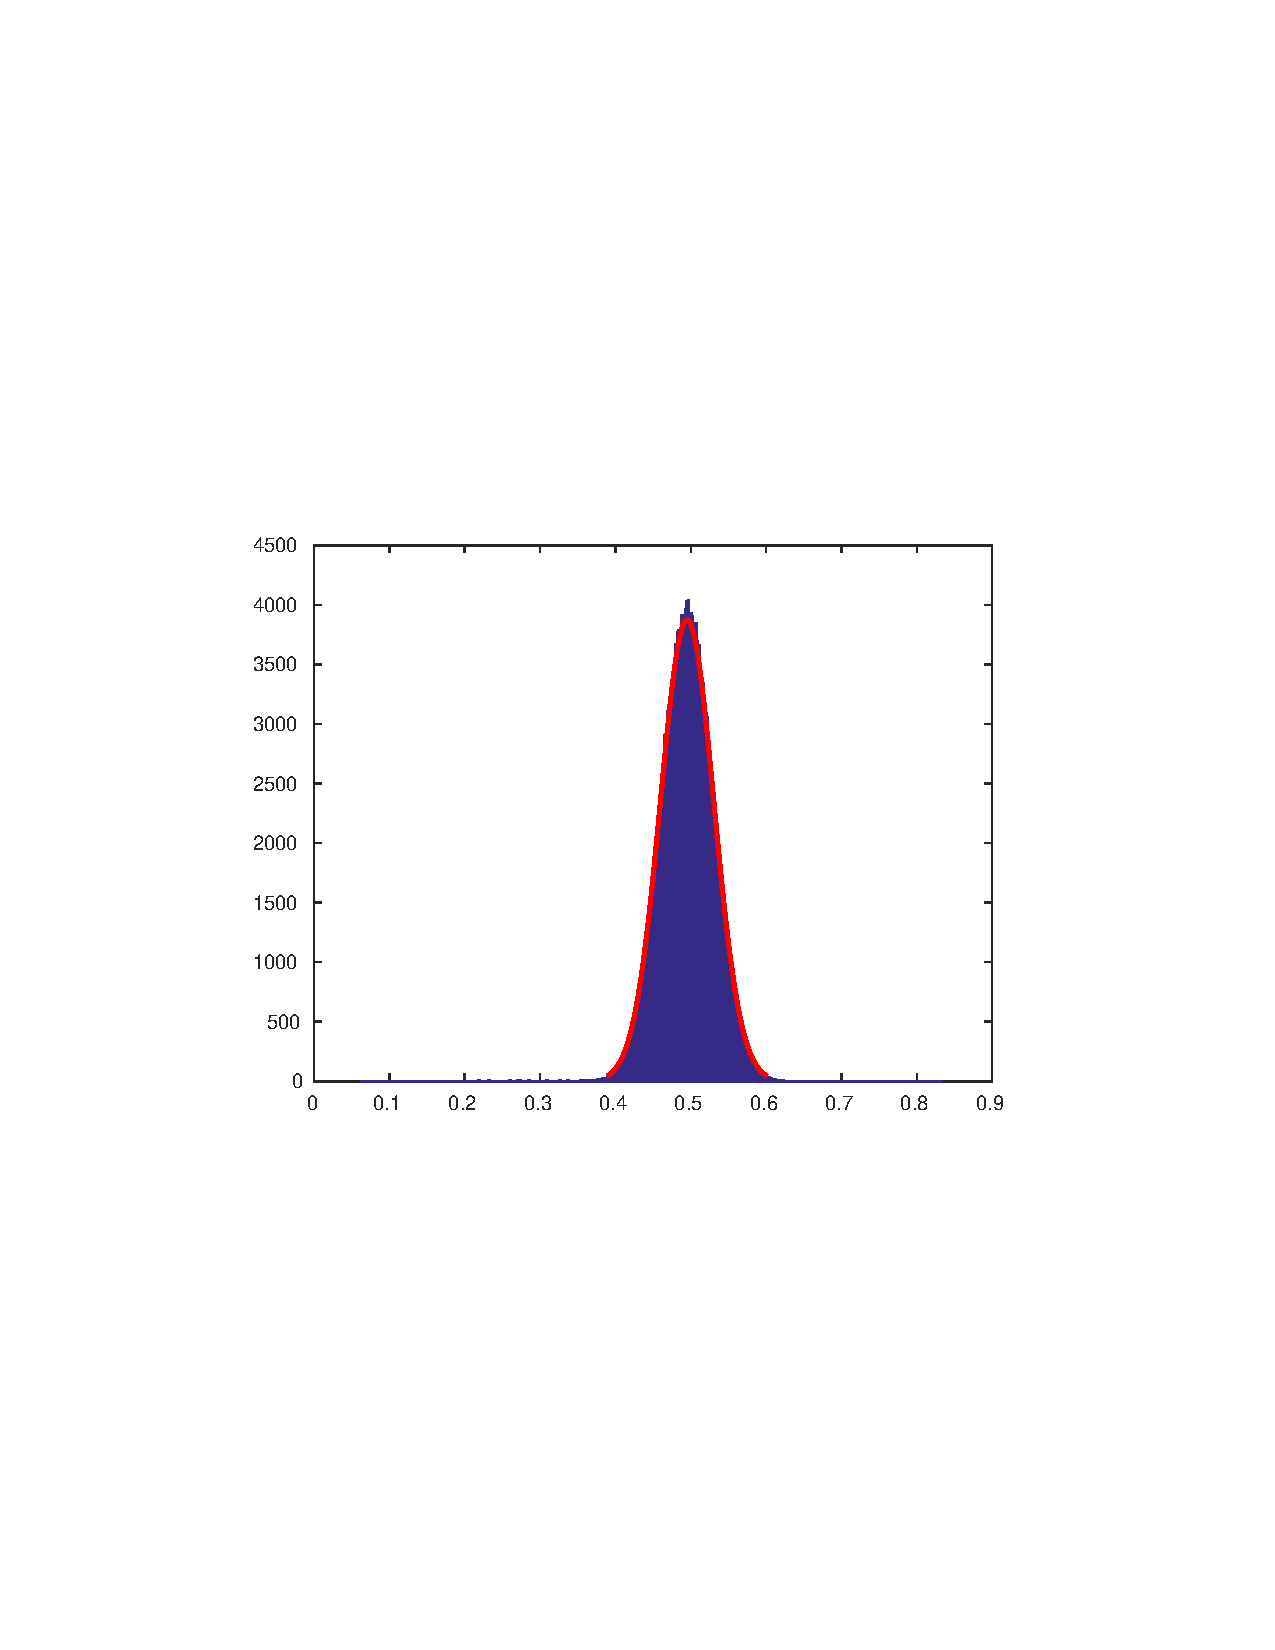
\includegraphics[width=1.0\textwidth]{imgs/theta2.pdf}
	\caption{\footnotesize Histograma de la variable $\theta_2$. La linea roja es una aproximacion con una distribución normal.}
\end{minipage}
\end{figure}

\subsection{Correlaciones}

Creimos que podía ser interesante ver el histograma conjunto entre las distribuciones de las monedas. Con esto pudimos visualizar como si en una distribución en cierto punto la moneda estaba cargada en la distribución de la otra moneda esta no lo estaba, esta situación genera los graficos formados alrededor del par de rectas que pasan por el 0.5.

\begin{figure}[H]
\begin{minipage}{0.5\textwidth}
 \centering
	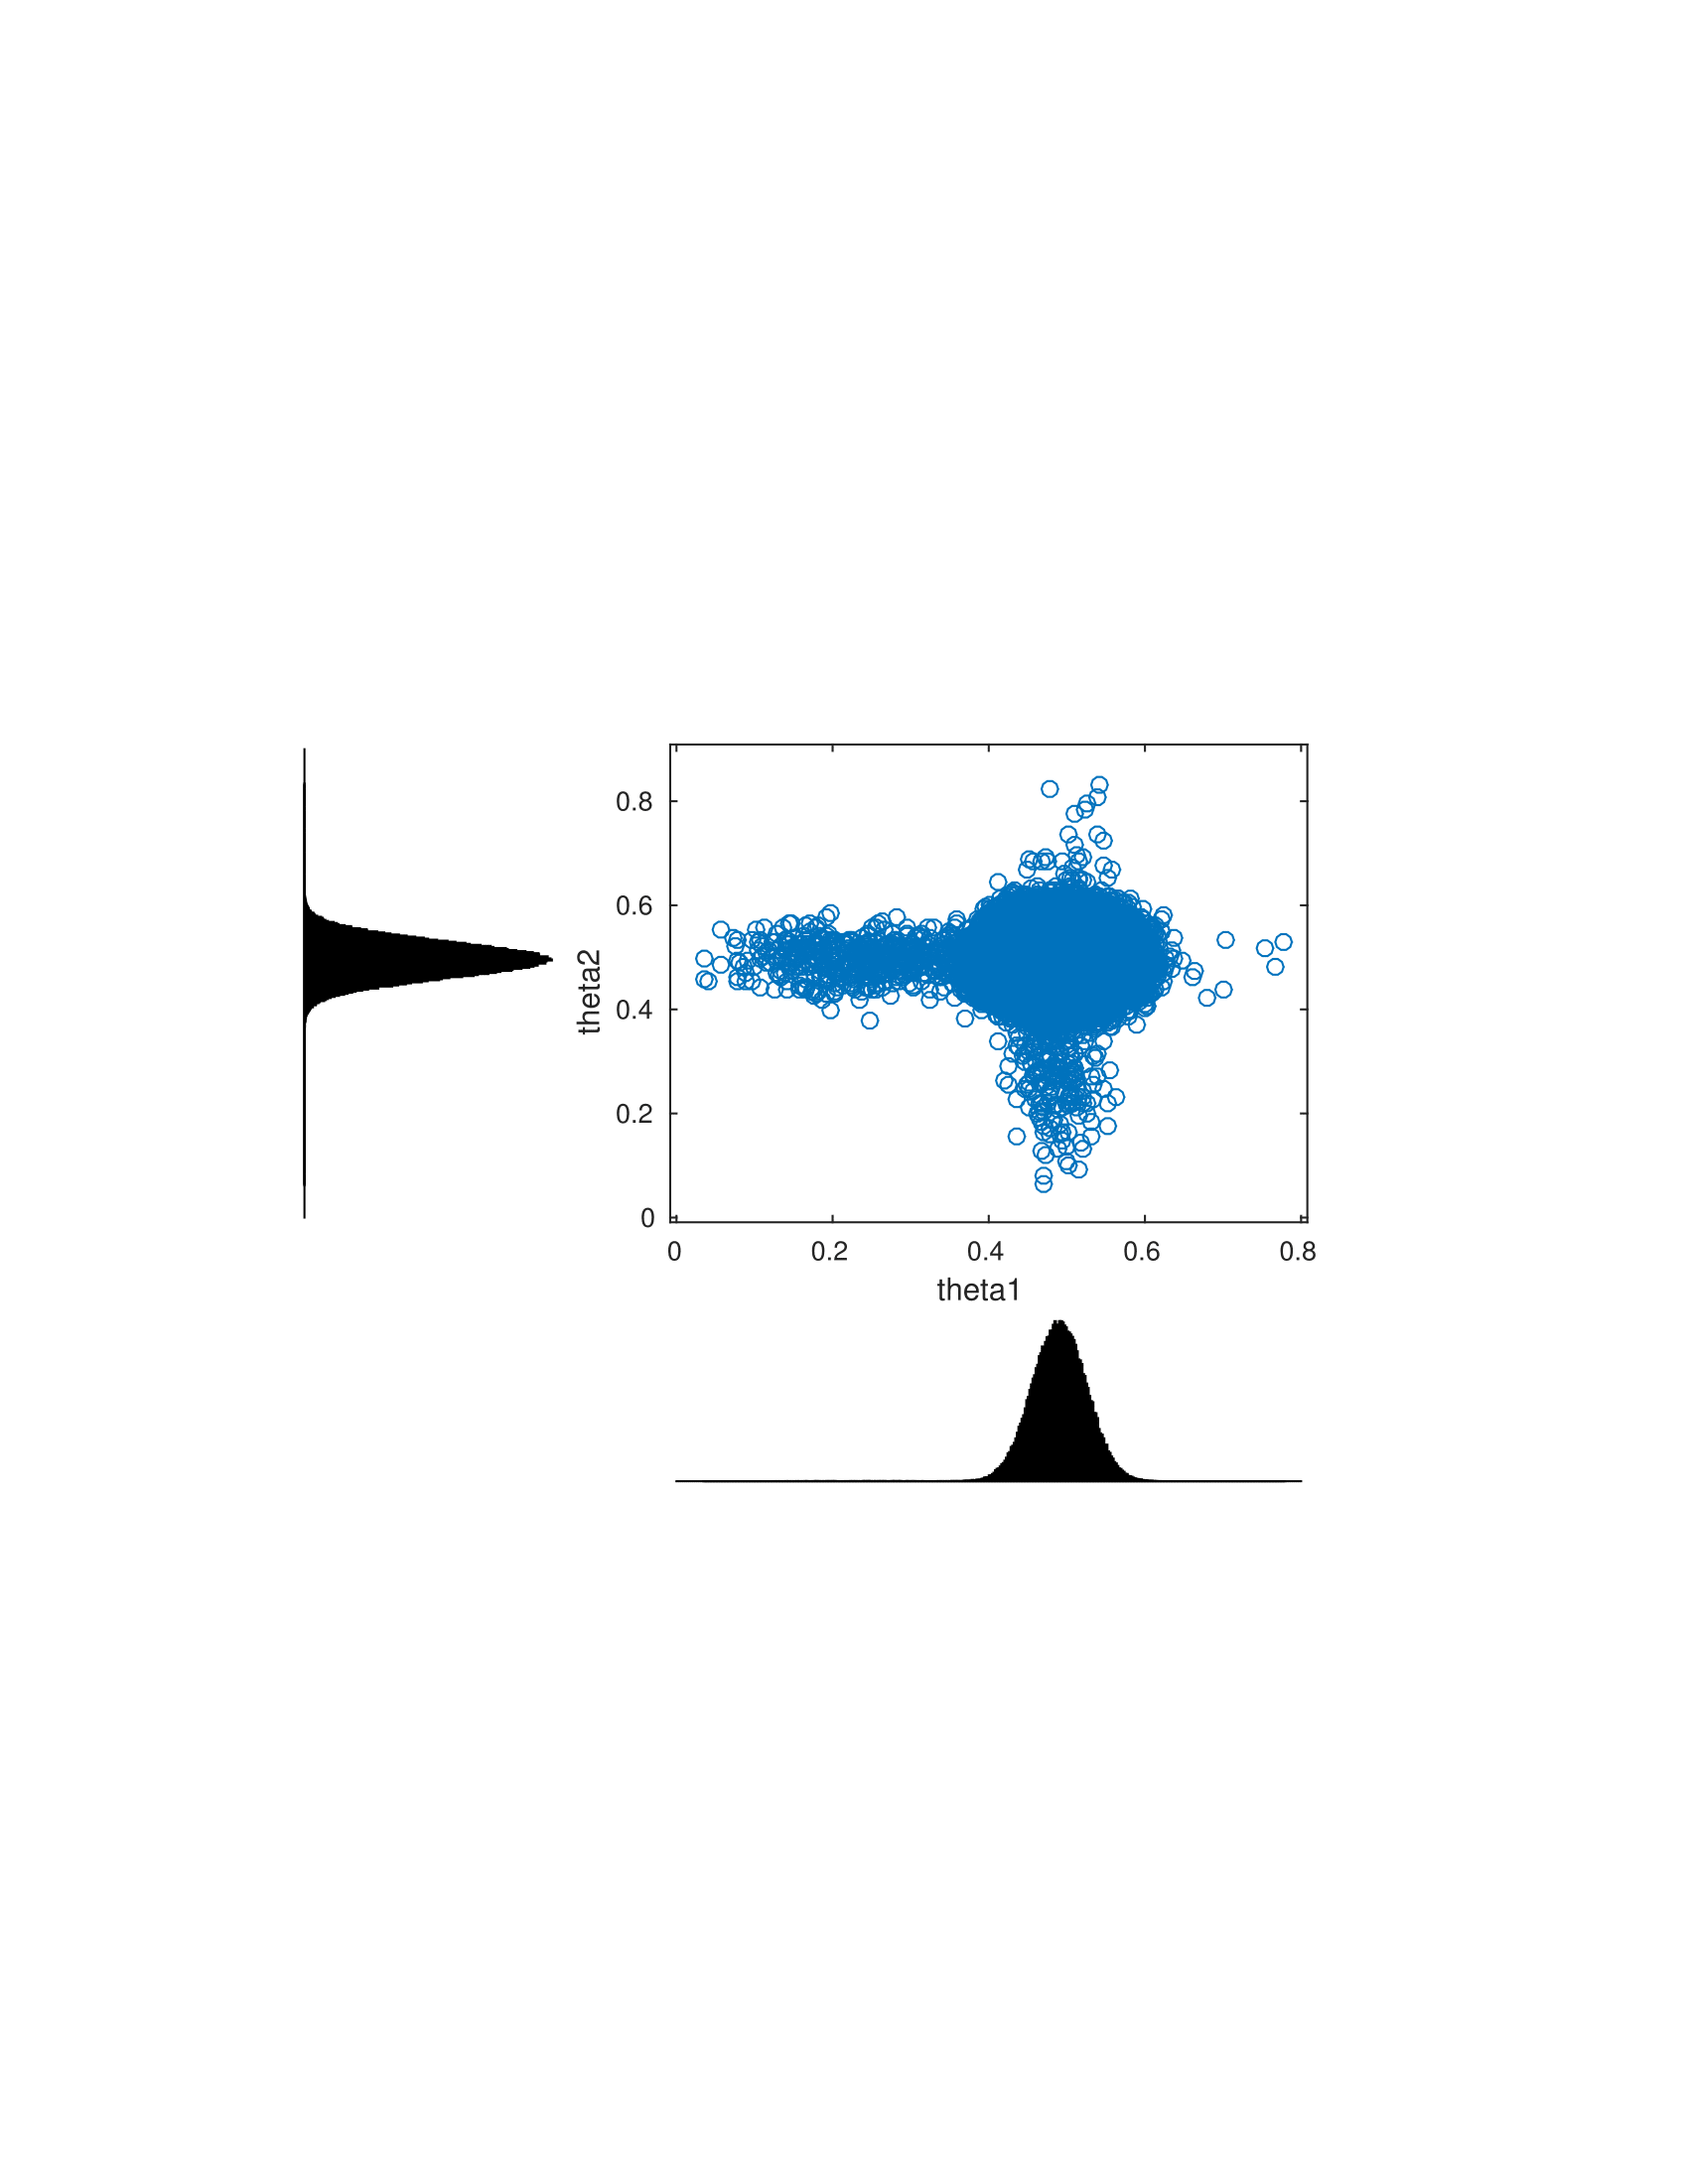
\includegraphics[width=1.0\textwidth]{imgs/theta1_2.png}
	\caption{\footnotesize Correlación entre $\theta_1$ y $\theta_2$.}
	\label{fig:problema2-promedio}
\end{minipage}
\begin{minipage}{0.5\textwidth}
 \centering
	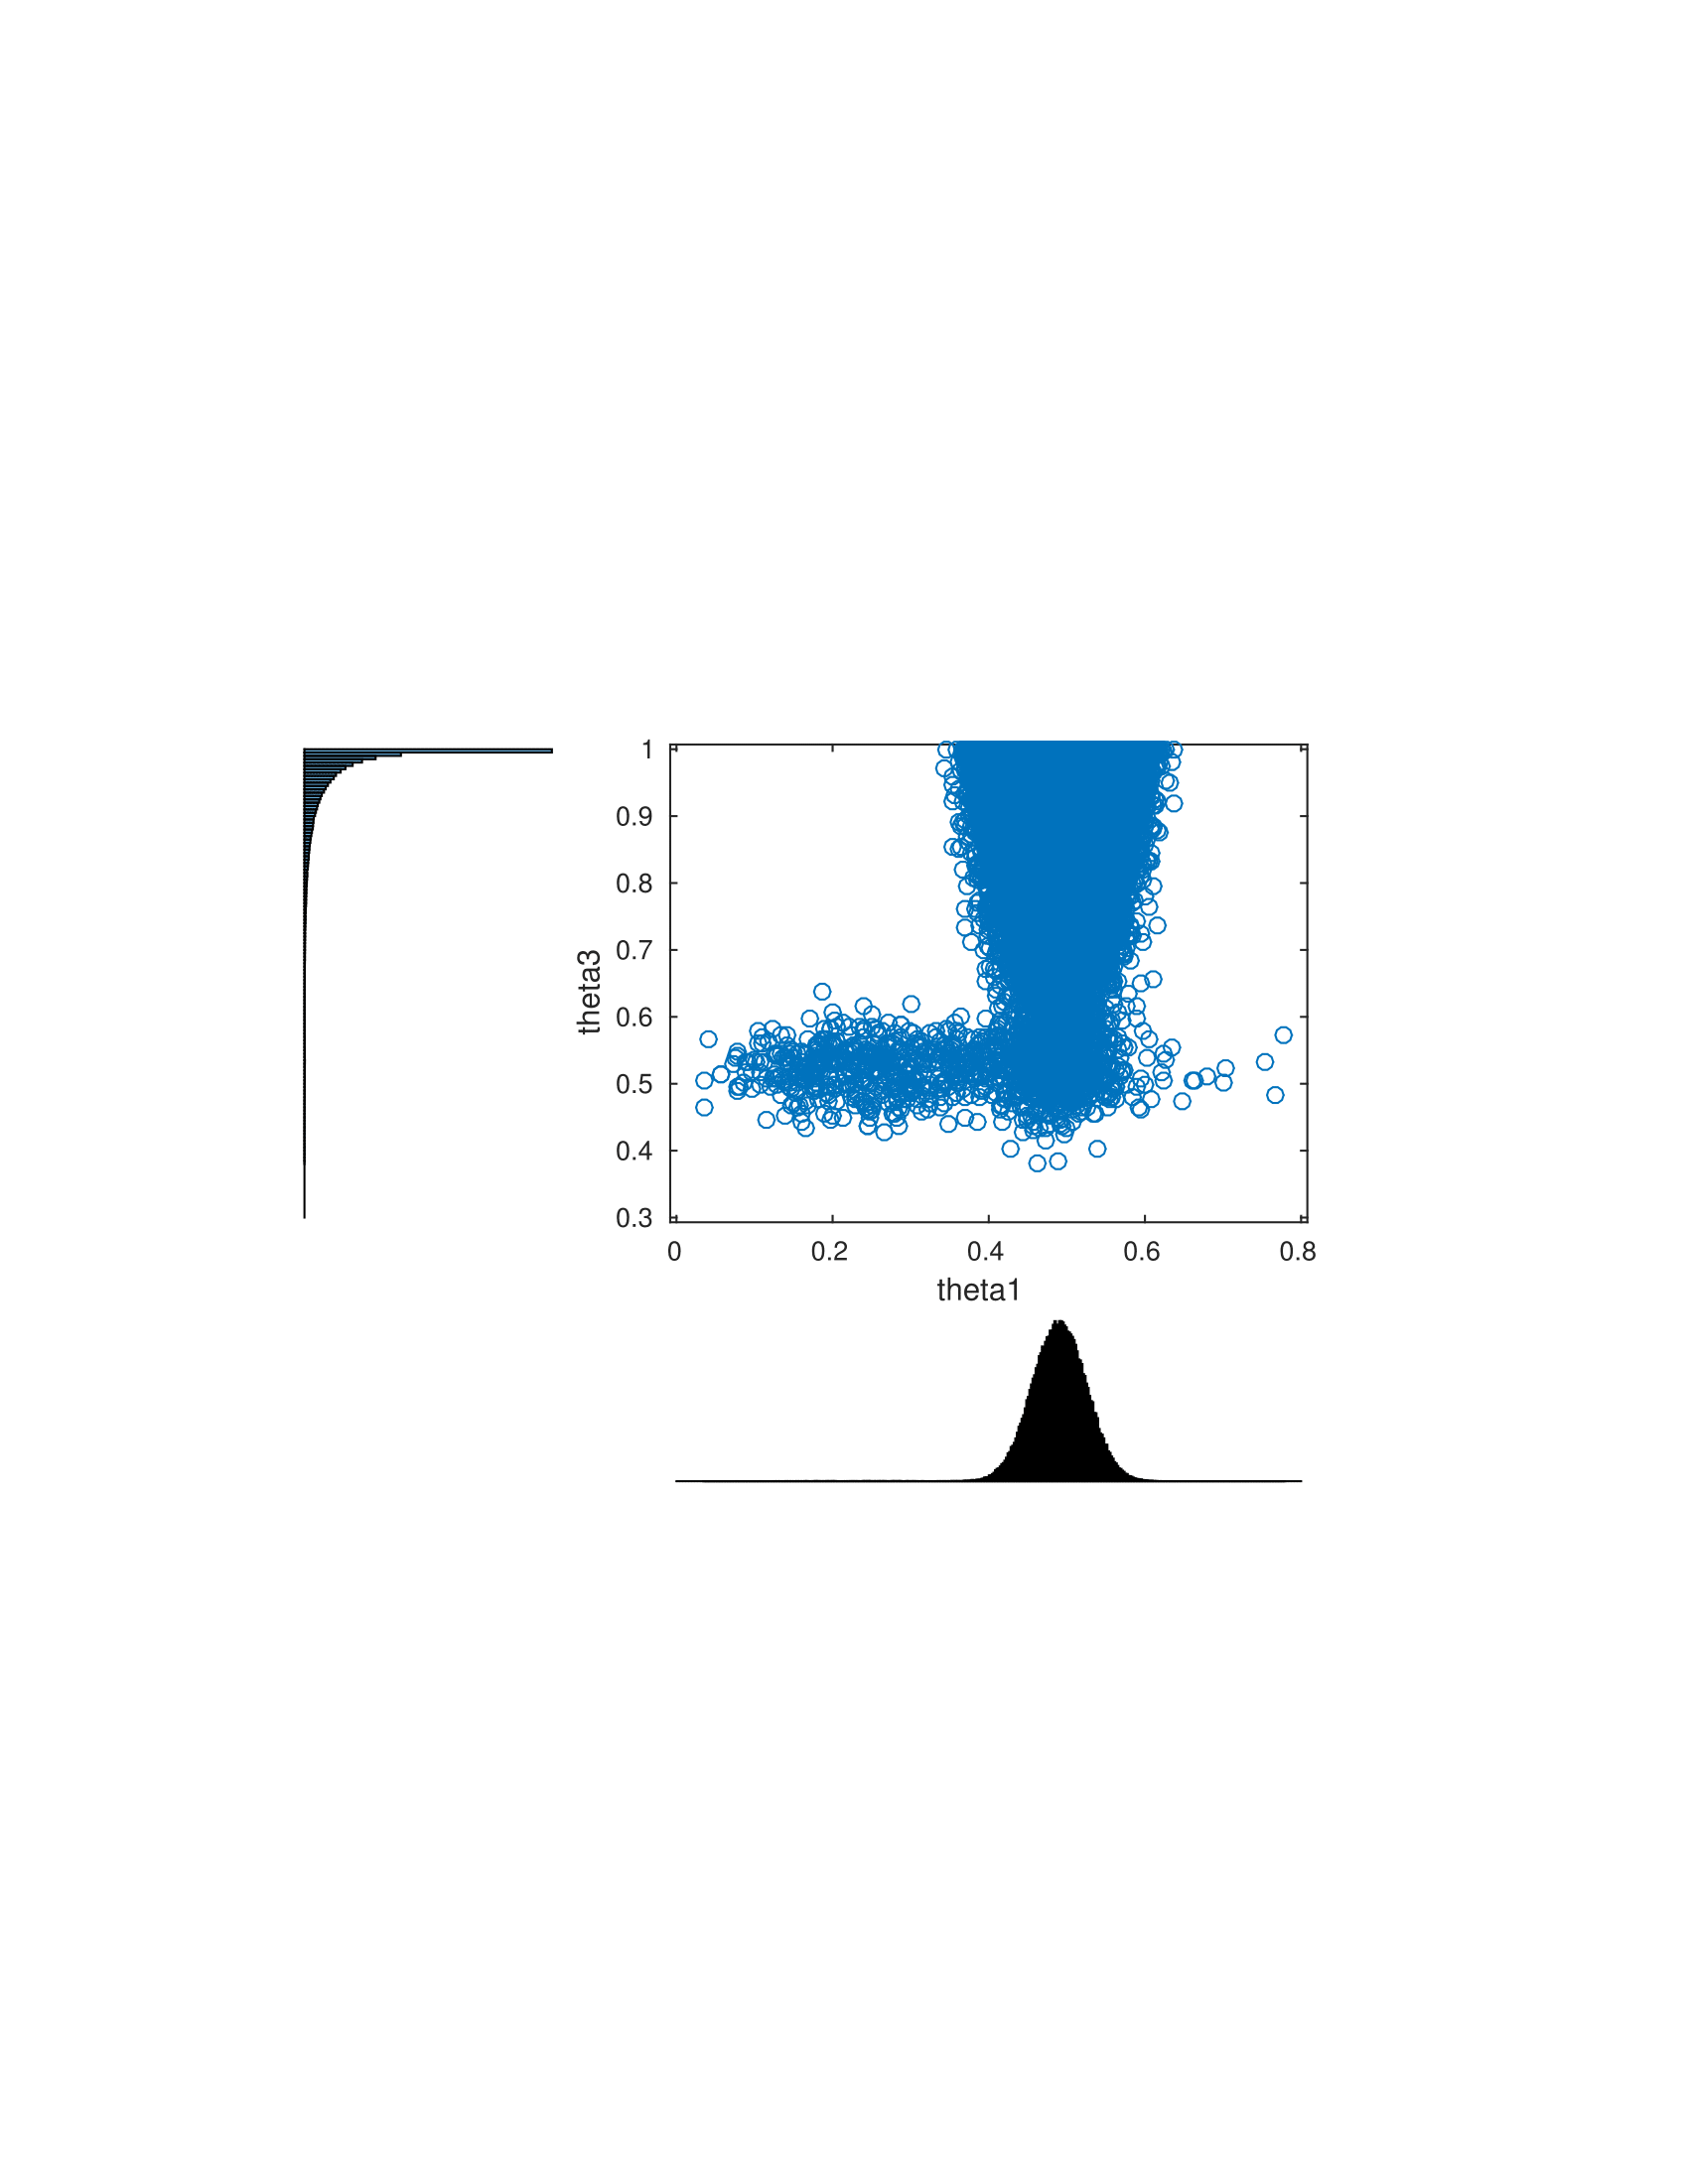
\includegraphics[width=1.0\textwidth]{imgs/theta1_3.png}
	\caption{\footnotesize Correlación entre $\theta_1$ y $\theta_3$.}
\end{minipage}
\end{figure}

\begin{figure}[H]
\centering
\begin{minipage}{0.5\textwidth}
	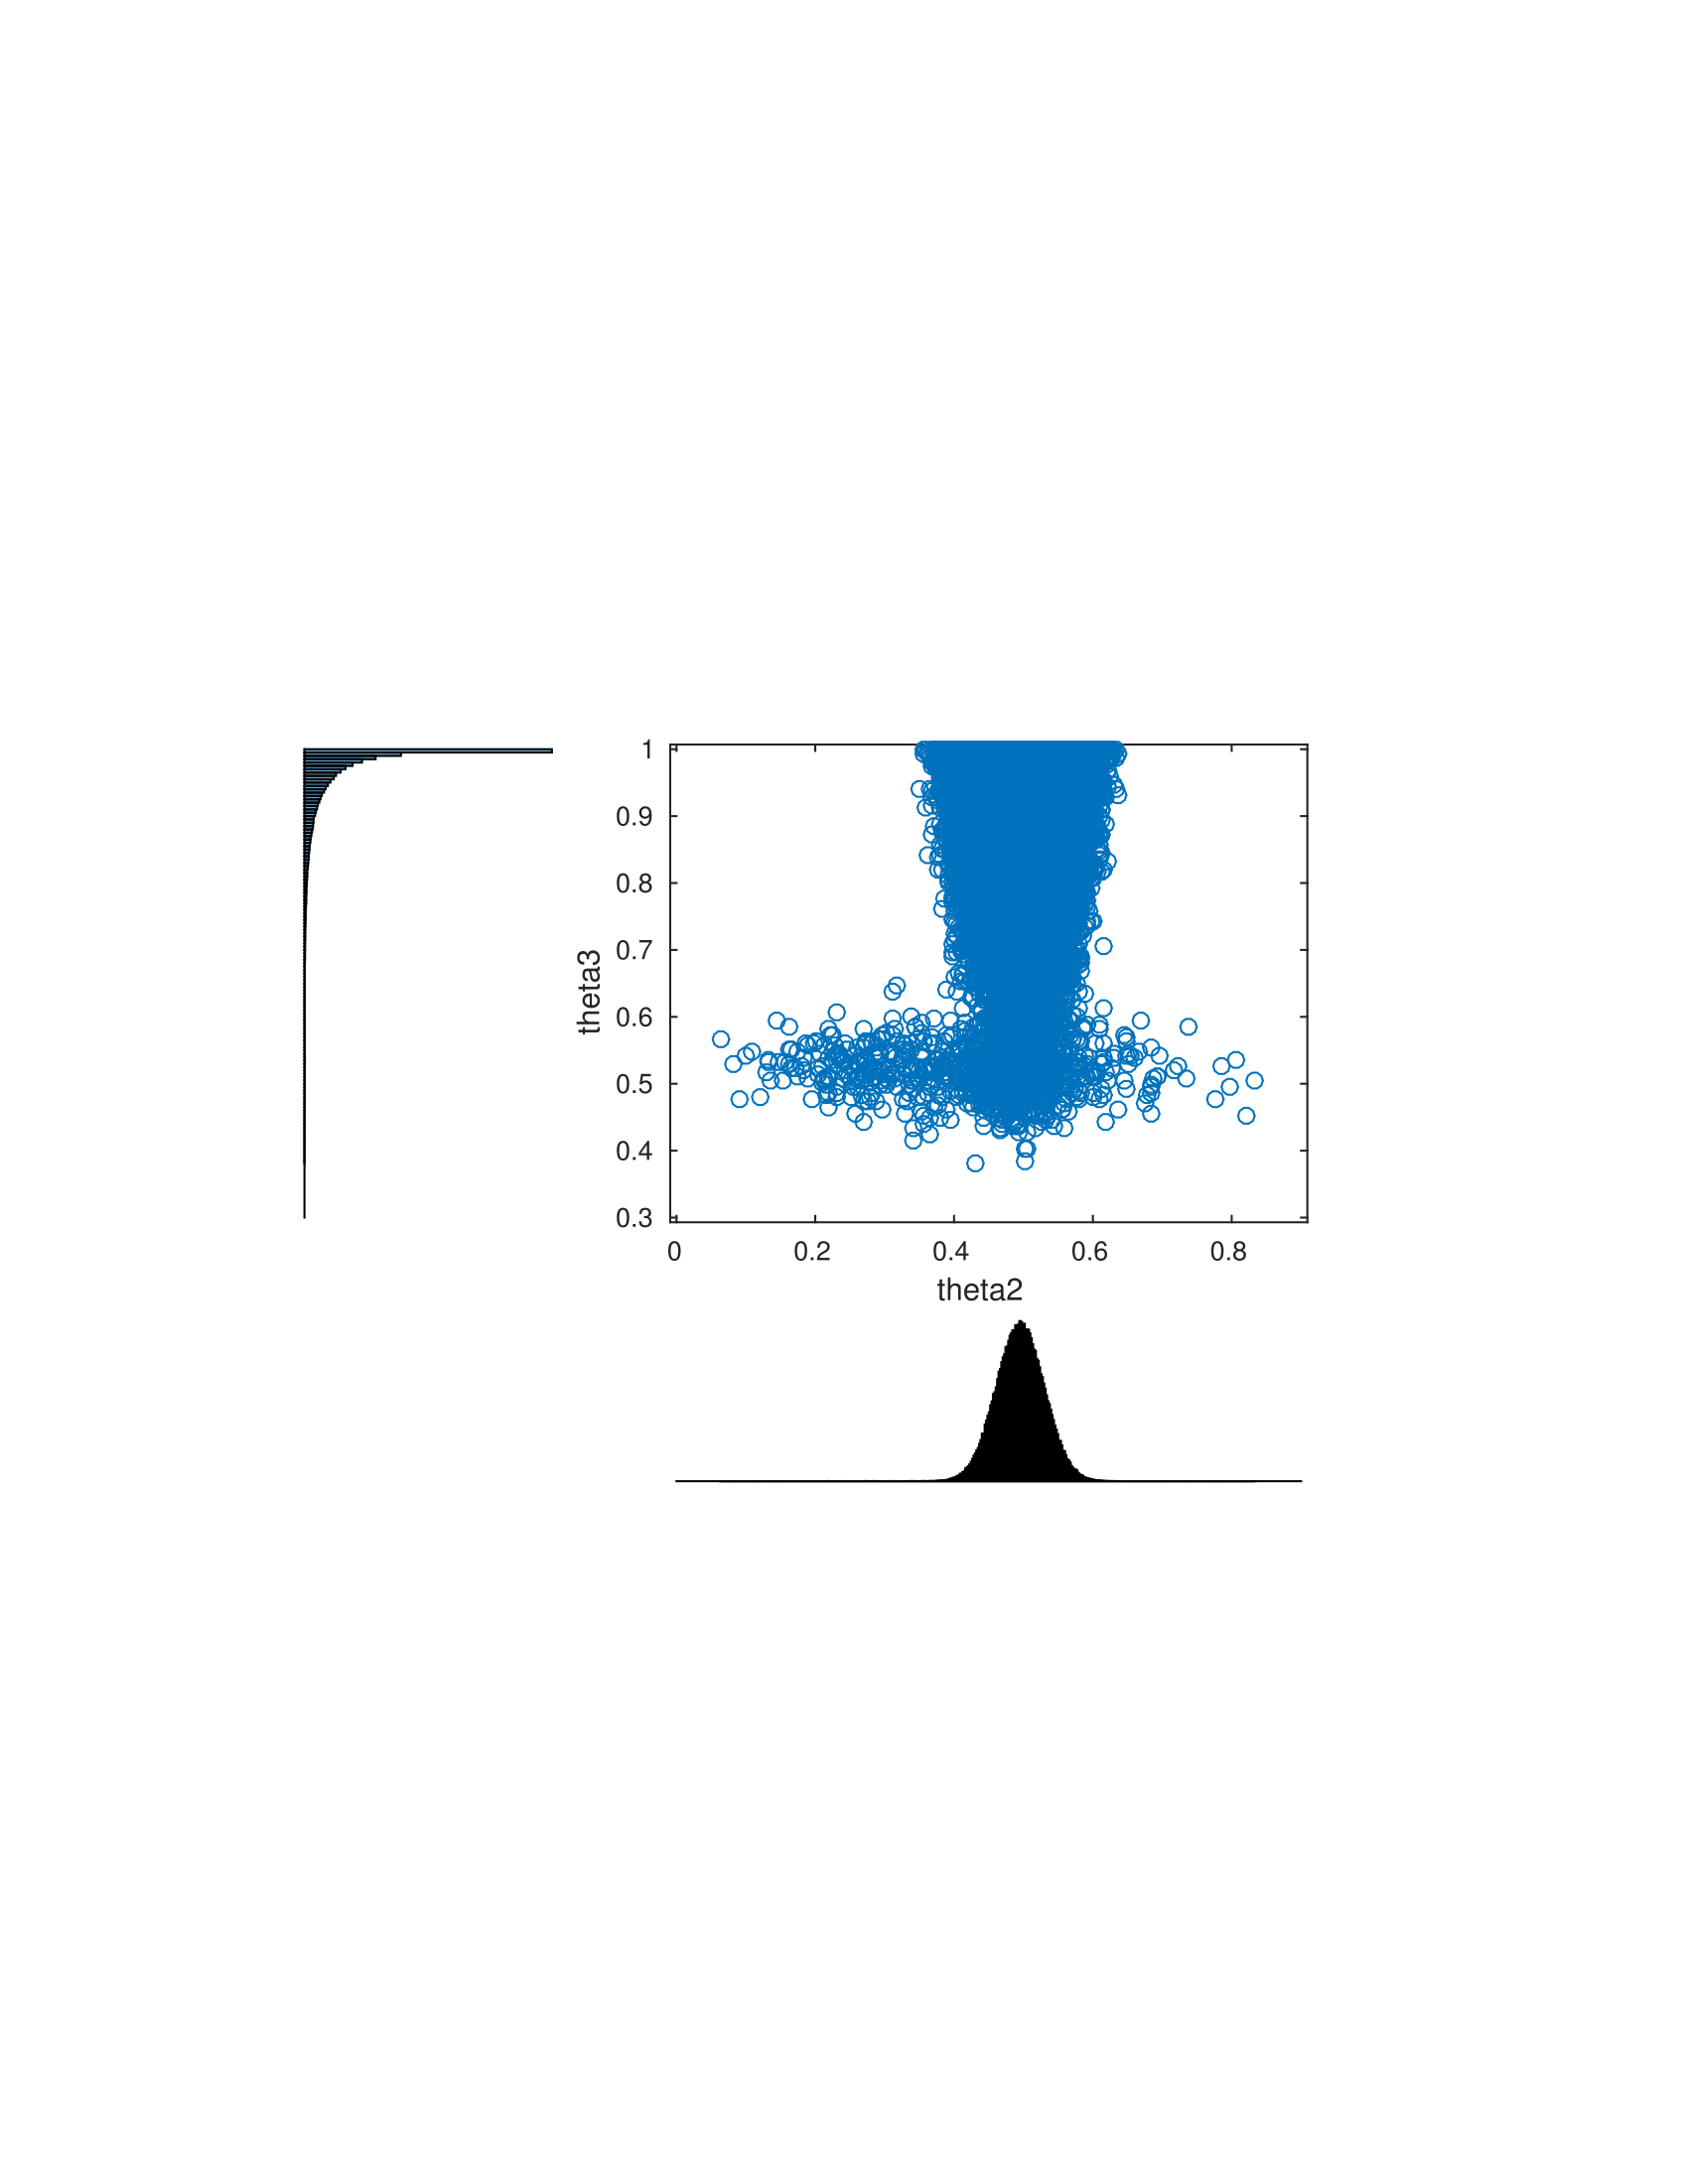
\includegraphics[width=1.0\textwidth]{imgs/theta2_3.png}
	\caption{\footnotesize Correlación entre $\theta_2$ y $\theta_2$.}
\end{minipage}	
\end{figure}


\subsection{Media y Desvío Standard}

En los resultados siguientes se puede ver un poco mas lo que esperabamos y habiamos verificado con los gráficos. Por ejemplo la variable $\alpha$ tiene una esperanza muy cercana a 3, ya que luego de hacer la inferencia con los datos obtenidos todo indica que la moneda número 3 es la cargada.

\begin{figure}[H]
\begin{minipage}{0.5\textwidth}
 \centering

$\mathop{\mathbb{E}} (\alpha) = 2.9907$

$\sigma (\alpha) = 0.1270$

$ \mathop{\mathbb{E}} (\theta_1) = 0.4899 $

$ \sigma (\theta_1) = 0.0368 $


\end{minipage}
\begin{minipage}{0.5\textwidth}
 \centering

$ \mathop{\mathbb{E}} (\theta_2) = 0.4951 $

$ \sigma (\theta_2) = 0.0354 $

$ \mathop{\mathbb{E}} (\theta_3) = 0.9523 $

$ \sigma (\theta_3) = 0.0680 $

\end{minipage}
\end{figure}

Las 2 primeras monedas parecen no estar cargadas con bastante seguridad ya que tienen una media de casi 0.5 con un desvío standard muy bajo. Esta situación creemos que es inducida por los datos obtenidos y la forma en que es armado el módelo donde solo una de las 3 monedas puede estar cargada.

\subsection{¿Esta cargada?}

Para calcular la probabilidad de que cada moneda este cargada, tomamos los 200000 samples de $\alpha$ generados por el algoritmo y calculamos la probabilidad de que salga un 1, 2 o 3. El resultado es el siguiente. 


P($\alpha$ = 1) = $\frac{694}{200000}$ = 0.0035

P($\alpha$ = 2) = $\frac{468}{200000}$ = 0.0023

P($\alpha$ = 3) = $\frac{198838}{200000}$ = 0.9942

Algo que nos sorprendió fue que según estos calculos la moneda 1 tiene mas chances de estar cargada que la 2 a pesar de que según los datos esta salió una menor cantidad de veces cara. Quedará como trabajo a futuro verificar si esto fue por el posible error en la aproximación del algoritmo o algun otro aspecto que no tuvimos en cuenta.